\newpage
\section{Resultados e Discussão}

Como resultado da simulação do circuito da Figura \ref{circuitoSimulado}, obtivemos os seguintes resultados:

\begin{figure}[H]
	\centering
	\caption{Circuito RLC paralelo simulado no Multisim Live.}
	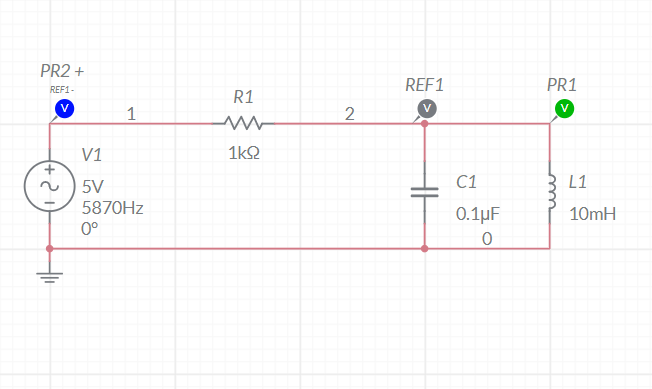
\includegraphics[width=15cm]{images/circuitoSimulado.png}
	\caption*{Fonte: Elaborado pelos autores.}
	\label{circuitoSimulado}
\end{figure}

\subsection{Filtro passa-faixa}
O módulo da função de transferência do circuito como filtro passa-faixa foi calculado para os valores de $\omega=0$, $\omega=\omega_n$ e $\omega\rightarrow\infty$, utilizando a equação \refeq{moduloFuncaoTransferencia}:
\begin{equation}
	\omega=0 \Rightarrow  |H(j\omega)|= 0
\end{equation}
\begin{equation}
	\omega=\omega_n \Rightarrow |H(j\omega)|= 1
\end{equation}
\begin{equation}
	\omega\rightarrow\infty \Rightarrow |H(j\omega)|= 0
\end{equation}

As frequências de corte $\omega_{c1}$ e $\omega_{c2}$, além da frequência de ressonância $\omega_0$ foram calculadas e convertidas para $Hz$, os resultados são apresentados a seguir, utilizando as equações \refeq{omegaC1}, \refeq{omegaC2} e \refeq{frequência de ressonância 2}:

\begin{equation}
	\omega_{C1}= -\frac{1}{2RC}+\sqrt{(\frac{1}{2RC})^2+\frac{1}{LC}}= 4302 Hz
\end{equation}
\begin{equation}
	\omega_{C2}=\frac{1}{2RC}+\sqrt{(\frac{1}{2RC})^2+\frac{1}{LC}}= 5894 Hz
\end{equation}
\begin{equation}
	\omega_0=\sqrt{\frac{1}{LC}}= 5036 Hz
\end{equation}

A conversão para $Hz$ foi dada devido a necessidade de utilizar as frequências dentro do simulador, cujo aceita apenas nesta unidade de medida.

\subsection{Filtro rejeita-faixa}
Quando o circuito se comporta como um filtro rejeita-faixa, sua função de transferência é diferente, pois agora o sinal de saída é dado pela tensão sob o resistor. Sendo assim, o módulo desta função para os diferentes valores de $\omega$ são calculados novamente, dessa vez utilizando a equação \refeq{moduloFuncaoTransferencia2}.
\begin{equation}
	\omega=0 \Rightarrow |H(j\omega)|= 1
\end{equation}
\begin{equation}
	\omega=\omega_n \Rightarrow |H(j\omega)|= 0
\end{equation}
\begin{equation}
	\omega\rightarrow\infty \Rightarrow |H(j\omega)|= 1
\end{equation}

As frequências de corte também foram calculadas para os novos valores, e também convertidas para Hz. A frequência de ressonância é a mesma para ambos os comportamentos do circuito, logo são utilizadas as equações \refeq{omegaC1}, \refeq{omegaC2} e \refeq{frequência de ressonância 2}:

\begin{equation}
	\omega_{C1}=\omega_0[-\frac{1}{2Q}+\sqrt{1+(\frac{1}{2Q})^2}]= 4299 Hz
\end{equation}
\begin{equation}
	\omega_{C2}=\omega_0[\frac{1}{2Q}+\sqrt{1+(\frac{1}{2Q})^2}]= 5891 Hz
\end{equation}
Sendo o fator de qualidade $Q= 3,162$, para ambos os filtros, de acordo com a equação \refeq{fator de qualidade}.

Um ponto importante a ser observado é que as frequências de corte do filtro rejeita-faixa são muito próximas dos valores calculados para o filtro passa-faixa, o que possibilita concluir que por ser o mesmo circuito, a faixa de frequência é a mesma.

\subsection{Simulação}

Com o circuito montado no software, a frequência dos sinais foi definida, à priori, como a frequência de corte $\omega_{C1}$ e ajustada até que o gráfico gerasse a resposta esperada:

Em torno deste valor de frequência inicia-se a faixa de frequência do circuito. Observa-se que a tensão no resistor e no conjunto LC são aproximadamente iguais, e espera-se que o comportamento seja o mesmo em torno da frequência $\omega_{C2}$. Simulando o circuito nestas condições:

\begin{figure}[H]
	\centering
	\caption{Resposta do circuito para a frequência $\omega_{c1}$.}
	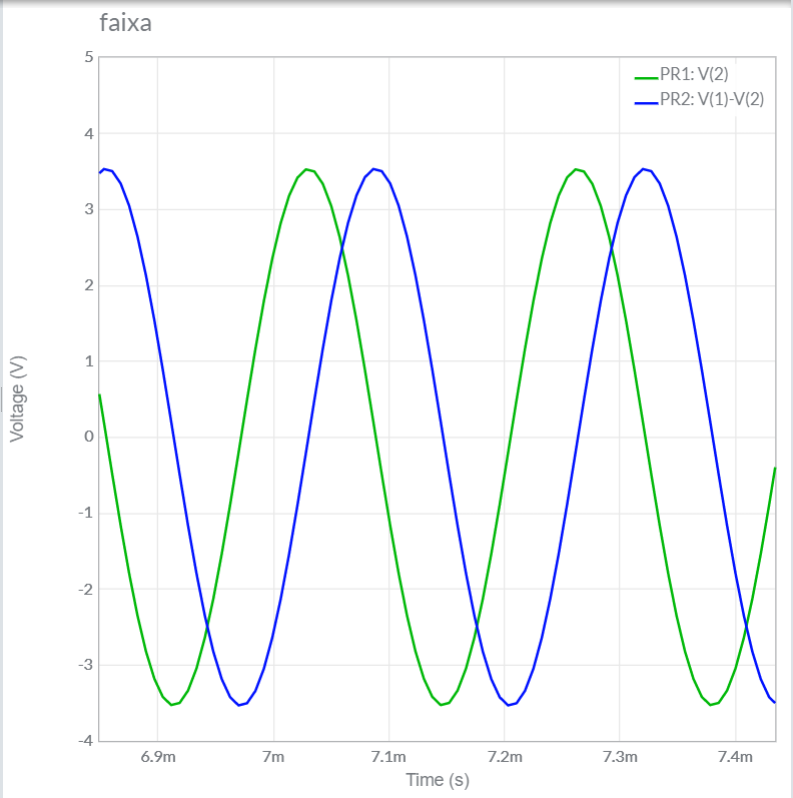
\includegraphics[width=10cm]{images/f_c1.png}
	\caption*{Fonte: Elaborado pelos autores.}
	\label{c1}
\end{figure}

\begin{figure}[H]
	\centering
	\caption{Resposta do circuito para a frequência $\omega_{c2}$.}
	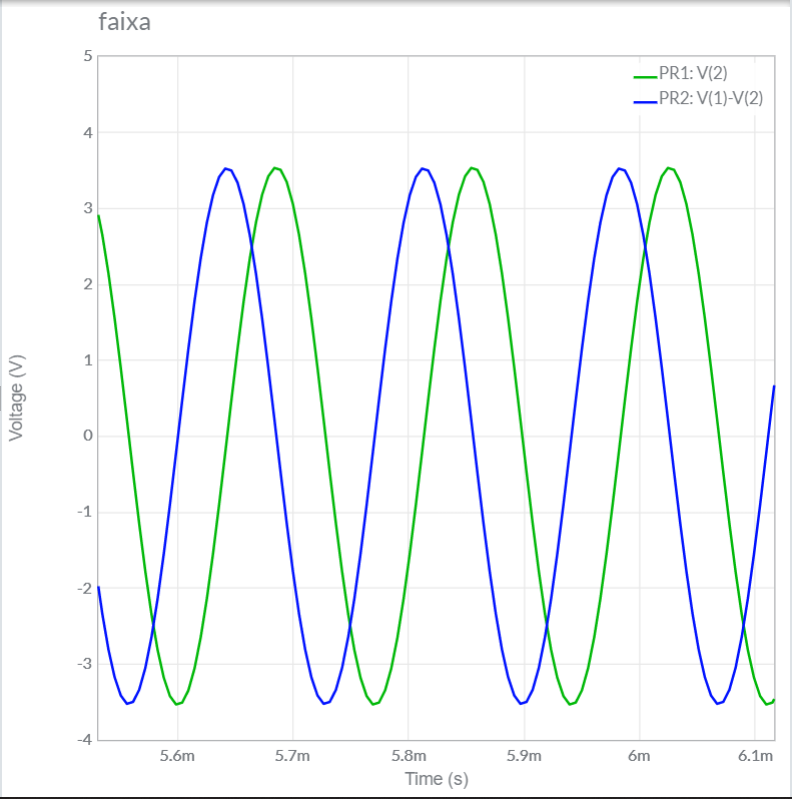
\includegraphics[width=10cm]{images/f_c2.png}
	\caption*{Fonte: Elaborado pelos autores.}
	\label{c2}
\end{figure}

O comportamento esperado é correto e novamente os valores de tensão no resistor e no conjunto LC são aproximadamente iguais, estes são apresentados na Tabela \ref{tabela} e devidamente comparados, tal como as respostas para a frequência de ressonância $\omega_0$, analisadas no gráfico da figura abaixo.

\begin{figure}[H]
	\centering
	\caption{Resposta do circuito para a frequência de ressonância $\omega_0$.}
	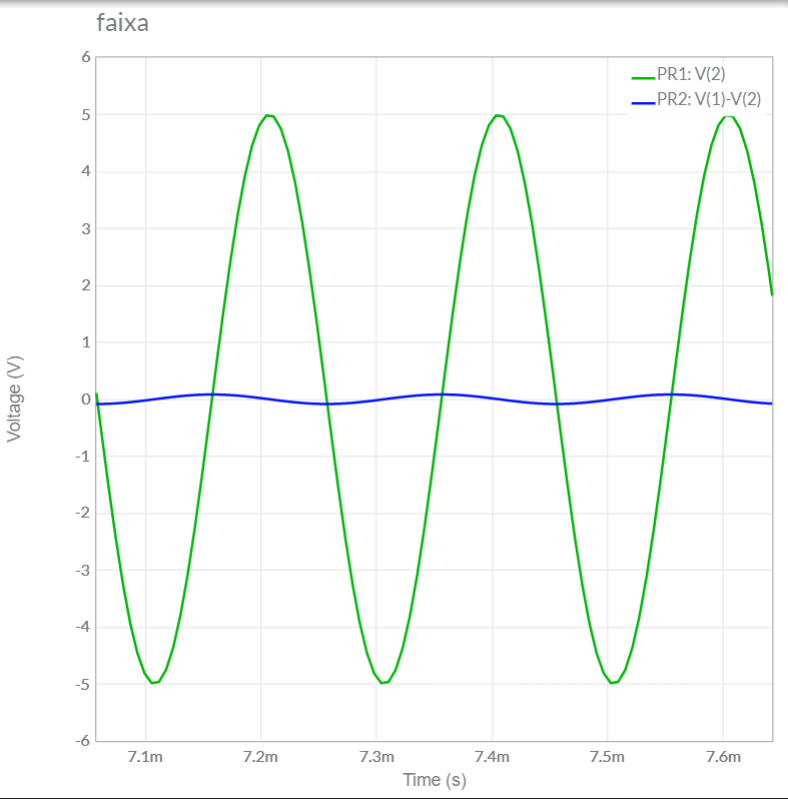
\includegraphics[width=10cm]{images/f_ressonancia.png}
	\caption*{Fonte: Elaborado pelos autores.}
	\label{ressonancia}
\end{figure}

Com o circuito respondendo à $\omega_0$, obtém-se o valor mínimo da tensão sobre o resistor, e o valor máximo da tensão sobre LC.

Para preencher as lacunas da tabela apresentada no roteiro, a operação foi repetida para mais alguns valores de frequência, e todas as respostas foram registradas, além do módulo da função de transferência para os dois diferentes filtros.

\begin{table}[H]
	\caption{Respostas do circuito RLC paralelo.}

	\begin{center}
		\resizebox{\textwidth}{!}{%
			\begin{tabular}{llllll}
				\hline
				\textbf{Frequência ($Hz$)} & \textbf{$v_i(t)$ ($V_{pp}$)} & \textbf{$v_R(t)$ ($V_{pp}$)} & \textbf{$v_C(t)$ ($V_{pp}$)} & \textbf{ $|H(j\omega)|$ (passa-faixa)} & \textbf{ $|H(j\omega)|$ (rejeita-faixa)} \\
				\hline
				785                        & 5                            & 4,9759                       & 0,0025                       & 0,0505                                 & 0,9987                                   \\
				2285                       & 5                            & 4,9184                       & 0,0089                       & 0,1780                                 & 0,9840                                   \\
				3285                       & 5                            & 4,7006                       & 1,7039                       & 0,3384                                 & 0,9410                                   \\
				3785                       & 5                            & 4,3722                       & 2,4216                       & 0,4802                                 & 0,8772                                   \\
				4285                       & 5                            & 3,5319                       & 3,5275                       & 0,6994                                 & 0,7147                                   \\
				4485                       & 5                            & 2,8935                       & 4,0748                       & 0,8075                                 & 0,5899                                   \\
				4785                       & 5                            & 1,4325                       & 4,7873                       & 0,9525                                 & 0,3044                                   \\
				5030                       & 5                            & 0,0064                       & 4,9843                       & 1,0000                                 & 0,0037                                   \\
				5370                       & 5                            & 1,8734                       & 4,6268                       & 0,9252                                 & -0,3796                                  \\
				5570                       & 5                            & 2,7280                       & 4,2488                       & 0,8414                                 & -0,5405                                  \\
				5870                       & 5                            & 3,5244                       & 3,5333                       & 0,7153                                 & -0,6988                                  \\
				6370                       & 5                            & 4,1159                       & 3,1502                       & 0,5537                                 & -0,8327                                  \\
				6870                       & 5                            & 4,6373                       & 2,0396                       & 0,4472                                 & -0,8944                                  \\
				7870                       & 5                            & 4,7514                       & 1,6703                       & 0,3237                                 & -0,9461                                  \\
				9370                       & 5                            & 4,8380                       & 1,2132                       & 0,2322                                 & -0,9727                                  \\
				\hline
			\end{tabular}}

	\end{center}
	\caption*{Fonte: Elaborado pelos autores.}
	\label{tabela}
\end{table}

A largura de banda do circuito é calculada experimentalmente e teoricamente (vide equação \refeq{beta}), tal como o erro percentual entre estes valores e entre as frequências também fora calculado.
\begin{equation}
	\beta_{t} = 10^4 Hz
\end{equation}
\begin{equation}
	\beta_{e} = 9,9538.10^3 Hz
\end{equation}
\begin{equation}
	\%E = 0,462\%
\end{equation}
Frequência de corte inicial:
\begin{equation}
	\%E = 0,395\%
\end{equation}
Frequência de corte final:
\begin{equation}
	\%E = 0,407\%
\end{equation}
Frequência de ressonância:
\begin{equation}
	\%E = 0,119\%
\end{equation}

\pagebreak